\chapter{绪论}
\citestyle{numbers}

作为现代人工智能的最重要的分之,人工神经网络(artificial neural network, ANN)近年来获得迅速发展。学术界不断提出新的神经网络理论,算法和结构,解决各类人工智能问题,提高网络性能和精度;工业界也相继将神经网络应用于目标检测,语音识别等领域。
然而随着神经网络解决的问题越来越复杂,神经网络也朝着规模越来越大,拓扑结构越来越复杂,层数越来越深的方向发展,因此神经网络需要庞大的存储资源,计算资源和能耗完成运算,这导致神经网络无法部署到嵌入式设备或者移动智能设备中。一个方面, 近些年来,研究者从算法,架构,物理等方面对神经网络进行深度压缩,其中稀疏(sparsity)被证明是其中最有效的一个策略,稀疏能够减少神经网络参数数量和计算量,使得稀疏神经网络能够部署到嵌入式设备中。另一个方面,研究者提出并设计了神经网络加速器,从而代替CPU/GPU完成神经网络运算,减少神经网络执行时间,降低能耗。然而,稀疏技术会使得神经网络的规则计算变为不规则,因此使得CPU,GPU和部分加速器不能从中获得性能提升;尽管有部分加速器能够支持稀疏,但是效果并不理想。因此本文提出了一种软硬件结合的方法处理稀疏神经网络的不规则形,从算法和架构设计的角度提出多种优化策略,显著提升处理稀疏网络的效果。

本章首先介绍神经网络算法的发展历程和神经网络处理平台的概况。然后介绍本文的主要研究内容及贡献。最后介绍本文的章节安排。

\section{神经网络算法发展历程}
人工神经网络的发展和成熟已经经过了四个时期,每个大约二十年,分别是1940年代和50年代,1960年代和70年代,1980年代和90年代,2000年至今。第一个时期主要完成了单个神经元的建模和学习。第二个时期主要建立了单层网络的模型和学习规则。第三个时期是多层神经网络蓬勃发展的时期,神经网络开始应用到多个领域。第四个时期神经网络的理论获得长足发展,同时深度神经网络在涌现同时被不断优化和改善,深度神经网络在图像处理,视频处理,自然语言处理等领域有着越来越广泛的应用。


\subsection{第一个时期(1940年代到50年代)}
第一个时期,研究者提出单个神经元的模型对应的学习规则。

学术界认为神经网络领域的先锋是~\citet{mcculloch1943logical},他首次正式提出了简洁又统一的神经元模型。
1949年,~\citet{hebb1963organizations, gerstner2002mathematical}首次提出了生物神经网络中存储信息的单位--突触(synapse),并提出了学习过程就是修改突触的过程这一条重要的规则,这条规则是目前许多网络学习训练的基础。

1952年,~\citet{hodgkin1952quantitative}利用动态方程建立了神经元脉冲发射的模型。

1956年~\citet{taylor1956electrical}使用联想记忆神经网络(associative memory)的方法模仿了许多不同的认知模型。

1958年,\citet{rosenblatt1958perceptron}提出了一套学习突触权值和神经元阈值的方法,最终完成了一个特定的信息处理任务,因此作者在这篇文章中提出了感知器(perceptron)的原型。

\subsection{第二个时期 (1960年代到70年代)}
第二个时期,研究者重点研究的是单层网络的模型和学习规则。

1960年,~\citet{widrow1960adaptive}采用最小二乘法(least mean-square algorithm)提出了线性适应元(adaptive linear element),这是一种自适应的模式分类神经元。

FitzHugh-Nagumo神经元模型~\cite{fitzhugh1961impulses}被广泛用于模拟感官系统中生物神经元的振荡行为。它使用相空间结合霍奇金-赫克斯利方程(Hodgkin-Huxley equations)的方法将神经纤维的生理状态划分为多个区域(包括活跃,压抑,增强,休息等),形成一个生理状态图,从而帮助研究者观察多种生理现象。

1967年~\citet{minsky1967computation}从自动机理论和计算理论的角度深入研究了研究了McCulloch和Pitts提出的神经元模型。1969年~\citet{minsky5paper}发现了单层感知机在处理信息任务时的局限性,并提出了多层感知机,然而多层感知机的学习规则在当时并没有深入研究,因此阻碍了神经网络的发展。

\citet{cainiello1961outline}提出当神经元受到的激励处于某个阈值时,该神经元不能被激活。1972年,~\citet{nagumo1972response}在此基础上提出了一种非线性的神经元模型,当一个恒定频率的脉冲序列作用于神经元时候,由于脉冲序列的振幅随时间减少,神经元被激活的频率也会随之减少。

\subsection{第三个时期(1980年代到90年代)}
第三个时期,研究者开始重点研究多层神经网络的模型和学习规则。在这个时期,贝叶斯方法,高斯过程,支持向量机(support vector machine,SVM)和多层神经网络都试图与生物模型结合,从而解释大脑的认知,学习,记忆等功能。

1982年,\citet{hopfield1982neural}将统计物理的概念应用于循环神经网络模型,提出了突触对称连接的神经网络,即Hopfield nets,这是80年代神经网络复兴的主要原因之一。这种简单优美的模型将记忆储存为激活值中的模式。

之后,广义Hopfield网络(generalized Hopfield network,GHN)用多层神经网络代替了单层神经网络结构,该结构被不断研究和发展。~\citet{zurada1996generalized}证明GHN拥有多个稳定状态,能够保证原始Hopfield网络的稳定性。因此,各种基于GHN的网络不断被提出来解决不同的问题。

虽然主成分分析(principal components analysis,PCA)早在1901年被提出,它主要用于生物领域的线性回归分析,但是它直至1980年代才被广泛应用于神经网络领域,PCA能够降低数据维度,快速发现子空间中的最大方差。

1984年,~\citet{hindmarsh1984model}提出了henomenological model,它能够将复杂的微分方程减少到三个,但是这个相对简单的模型能够解释合理地神经元的震荡现象。

1985年,~\citet{ackley1985learning}提出了玻尔兹曼机(Bolzmann machine),它在信息理论方面有着方唱广泛的应用。玻尔兹曼机基于模拟退火算法(simulated annealing),产生周期性的随机网络,并且根据玻尔兹曼分布模拟产生输入信号。其中,~\citet{kirkpatrick1983optimization, vcerny1985thermodynamical}提出的模拟退火算法是一个基于统计力学来解决优化问题的方法。

1986年,~\citet{rumelhart1986learning}应用反向传播(back propagation,BP)算法来训练神经网络,从而解决了~\citet{minsky5paper}提出的多层感知机难以进行学习的问题。由于多层前馈网络的训练经常采用BP算法,人们也常把将多层前馈网络直接称为BP网络。BP网络能学习和存贮大量的输入-输出模式映射关系,而无需事前揭示描述这种映射关系的数学方程。它的学习规则是使用最速下降法(梯度下降法),通过反向传播来不断调整网络的权值和阈值,使网络的误差平方和最小。

90年代有不少研究将神经网络与概率理论相结合,从而诞生了统计机器学习方法(statistical machine learning)。\citet{mackay1992practical, bishop1995neural}将贝叶斯技术(Bayesian technique)应用于到神经网络中,用于解决推理,回归和分类等问题。同时,~\citet{williams1996gaussian}将高斯方法论(methodology of Gaussian )引入到神经网络领域。

1998年,\citet{vapnik1998statistical}提出了支持向量机(SVM)。SVM的基本想法是利用kernel产生非线性表示,从而解决非线性的问题。支持向量机在模式识别,回归和密度估计等方面有着非常广泛的应用,尽管SVM被有些研究者被认为是神经网络的一个分支,但是学术界普遍认为SVM和神经网络是两个不同的领域。


\subsection{第四个时期(2000年代至今)}

第四个时期,研究者开始研究深度神经网络(deep neural network, DNN),深度神经网络由多种不同的层构成,输入数据依次通过各个层被逐层处理,最终被分类, 识别或者检测。深度神经网络还包括卷积神经网络(convolutional neural network, CNN)和循环神经网络(recurrent neural network);前者广泛应用于计算机视觉~\cite{krizhevsky2012imagenet,simonyan2014very, ren2015faster},而后者广泛应用于语音处理~\cite{hinton2012deep, amodei2015deep, ze2013statistical}或者自然语言处理~\cite{conneau2016very}。
最近轰动全球的成果就是谷歌旗下的Deep Mind团队所设计的Alpha Go~\cite{moyer2016google},在围棋上先手战胜李世石和柯杰等顶级棋手。下面主要介绍神经网络在图像处理领域和目标检测领域的应用和发展,然后介绍神经网络的低功耗技术。

\subsubsection{神经网络在图像分类领域的应用}
在2012年,深度神经网络在图像识别和分类领域领域取得了非常优秀的效果,~\citet{krizhevsky2012imagenet}提出的AlexNet网络结构,AlexNet是一个8层的网络结构,由5个卷积层和3个全连接层组成,
在ILSVRC-2012上top-5的错误率为$34.2\%$。 研究者发现,深度神经网络比浅层神经网络能够提取更高级的特征,网络的精度也就越高。因此,~\citet{simonyan2014very}提出了VGG网络,VGG共由16个层构成,其中包括13个卷积层和3个全连接层,在ImageNet数据集~\cite{deng2009imagenet}上top-5的错误率为$25.3\%$。

然而网络的层数不能无限增加,网络层数过多,不仅会导致梯度消失(vanishing gradient)或者梯度爆炸(exploding gradient)的问题,还会出现网络退化的问题,前者使得神经网络难以进行训练,后者导致神经网络的精度降低。~\citet{szegedy2015going}提出了GoogLenet网络,GoogLenet网络深度达到了22层,它最主要的特征在于使用了inception结构,从而更好地利用了网络中的计算资源,并且在不增加计算负载的情况下,增加网络的宽度和深度。inception结构的主要思想在于卷积视觉网络中一个优化的局部稀疏结构怎么样能由一系列易获得的稠密子结构来近似和覆盖。为了避免patch对齐问题,因此限制了inception结构中滤波器的大小为1x1,3x3,5x5。最终GoogleNet网络在ImageNet数据集上top-5的错误率为$26.7\%$。~\citet{he2016deep}在2016年提出了深度残差网络(deep residual network),在ImageNet中斩获图像分类、检测、定位三项的冠军。ResNet通过shortcut的结构进行参差学习,解决了增加深度带来的退化问题,这样能够通过单纯地增加网络深度,来提高网络性能,作者在ImageNet上实验了一个152层的残差网络,比VGG深8倍,最终取得了$3.57\%$的top-5错误率。

\subsubsection{神经网络在目标检测领域的应用}
除了图像识别/分类,深度神经网络在目标检测领域也有广泛应用,并且取得了非常理想的效果。2014年,~\citet{girshick2014rich}提出了RCNN网络解决目标检测问题,RCNN的主要思想是将检测问题转化成为分类问题。
RCNNN使用region proposal来得到有可能得到是object的若干(大概$10^3$量级)图像局部区域,然后把这些区域分别输入到CNN中,得到区域的feature,再在feature上加上分类器,判断feature对应的区域是属于具体某类object还是背景。当然,RCNN还用了区域对应的feature做了针对bounding box的回归,用来修正预测的bounding box的位置。RCNN在VOC2007上的mAP是$58\%$左右。

RCNN存在着重复计算的问题(proposal的region有几千个,多数都是互相重叠,重叠部分会被多次重复提取feature),于是~\citet{girshick2015fast}借鉴~\citet{he2014spatial}的SPP-net的思路提出了Fast-RCNN,跟RCNN最大区别就是Fast-RCNN将proposal的region映射到CNN的最后一层卷积层的feature map上,这样一张图片只需要提取一次feature,大大提高了速度,也由于流程的整合以及其他原因,在VOC2007上的mAP也提高到了$68\%$。

Fast-RCNN的速度瓶颈在Region proposal上,于是~\citet{ren2015faster}提出了Faster-RCNN,将Region proposal也交给CNN来做。Fater-RCNN中的region proposal netwrok实质是一个Fast-RCNN,这个Fast-RCNN输入的region proposal的是固定的(把一张图片划分成n*n个区域,每个区域给出9个不同ratio和scale的proposal),输出的是对输入的固定proposal是属于背景还是前景的判断和对齐位置的修正(regression)。Region proposal network的输出再输入第二个Fast-RCNN做更精细的分类和Boundingbox的位置修正。Fater-RCNN速度更快了,而且用VGG net作为feature extractor时在VOC2007上mAP能到$73\%$。

神经网络在目标检测领域还在持续发展,研究这不断提出新的网络和方法如Mask-RCNN~\cite{he2017mask},YOLO~\cite{redmon2016you}来加快网络运行速度和精度。


\subsubsection{神经网络的低能耗技术}
随着神经网络的应用越来越广泛,神经网络的拓扑结构朝着规模不断扩大,层数不断加深的方向发展,因此未来的大规模网络很难部署到嵌入式系统中。很多研究人员致力于减少神经网络的参数规模,从而减少对存储资源,计算资源和带宽的需求,加快神经网络运行速度,降低神经网络的能耗。研究者提出了许多方法来解决这个问题,主要可以分为低精度计算和压缩技术。

低精度计算主要将神经元的权值或神经元进行低比特量化,从而降低网络存储需求和运算能耗。低精度量化包括16比特定点量化~\cite{gupta2015deep},8比特量化~\cite{dettmers20158},二元权值量化~\cite{courbariaux2015binaryconnect},三元权值量化~\cite{rastegari2016xnor},2的幂次等形式的量化~\cite{zhou2017incremental}。

神经网络的压缩技术采用剪枝,矩阵分解等方法直接减少神经网络中参数数量。剪枝技术~\cite{reed1993pruning, lecun1989optimal, miche2010op, han2015learning}能够修剪神经网络中不必要的链接,如果神经元或者权值满足某些条件,那么这些神经元/权值将会被修剪,从而降低网络的复杂性和过拟合,最终获得具有良好泛化性能的精简神经网络。矩阵分解技术则采用矩阵因式分解~\cite{denton2014exploiting, lebedev2014speeding}的对权值矩阵或者卷积核进行分解,在保持模型规则计算的情况下,实现神经网络压缩和加速。

\section{神经网络计算平台发展}

主流的神经网络计算平台是通用处理器,即CPU和GPU。然而CPU的性能并不能满足实际的需求,而GPU的的能耗过高。因此研究者开始为神经网络算法设计专用的加速器,使得神经网络算法在加速器上既能够满足高性能的需求,又能够满足低能耗的需求。目前有两个流行的加速平台,分别是可编程逻辑门阵列(field-programmable gate array,FPGA)和专用集成电路(application specific integrated circuit , ASIC)。

\subsection{通用处理器CPU和GPU}
CPU~\cite{chakradhar2010dynamically, vanhoucke2011improving}和GPU~\cite{farabet2009cnp, scherer2010accelerating, ciresan2011flexible, coates2013deep}是两个完成神经网络运算的通用平台。同时,在CPU和GPU上,有许多针对神经网络的高级编程框架,如Caffe~\cite{jia2014caffe},Tensorflow~\cite{abadi2016tensorflow},MXNet~\cite{chen2015mxnet},使得用户能够方便地将神经网络算法部署到CPU和GPU上进行计算。

\citet{vanhoucke2011improving}在CPU上对神经网络算法进行了优化,包括循环展开,使用SIMD指令并行累加,调整数据保证内存对齐,使用8比特量化减少内存占用等,最终获得了4倍的性能提升。CPU集群更能够满足大规模网络应用的性能需求。谷歌提出了由数万个CPU组成的神经网络训练框架——DistBelief~\cite{dean2012large},并用它来训练由数十亿个参数构成神经网络,训练数据集为1000万张$200\times 200$的图片,训练事件长达3天时间,最终在ImageNet数据集上获得了$15.8\%$的错误率。

在CPU集群中,由于核之间的通信延迟高,带宽低,因此核之间的通信会成为整个系统的瓶颈。GPU采用完全不同的体系结构,它采用单任务多数据(single program multiple data, SPMD)框架,兼有分布式存储和共享内存的优点,具有非常高的并行性。因此,GPU对于计算密集(compute intensive)型应用,如CNN和DNN,性能完全超过CPU。2004年,~\citet{oh2004gpu}成功地将神经网络部署到GPU进行运算。2010年,~\citet{scherer2010accelerating}使用CUDA框架将大规模CNN部署到GPU,在训练过程中,每一个block负责一个batch运算,每一个thread负责一个权值的运算,同时利用共享内存重用输入数据或错误信号,从而大大提高内存利用率。
更进一步的,不少研究者开始全面探究如何使用GPU加速机器学习算法。

然而,CPU和GPU在处理神经网络时的效率并不高,因为这些通用处理器首先考虑的是通用性和普遍性,许多处理逻辑(包括计算和存储)对神经网络计算的支持并不理想。从计算的角度考虑,通用处理器只支持基本的计算,复杂的算术运算是通过一系列的基本计算组成,因此寄存器和内存频繁的数据交换不仅降低性能,还会带来大量的能耗。从存储的角度考虑,通用处理器采用冯·诺依曼体系中的层次化存储结构,缓存容量通常小于其他专用处理器,例如NVIDIA K20的片上缓存只有$1.5MB$,Intel E78880L的片上缓存不超过$50MB$。然后,随着神经网络的发展,神经网络的参数往十亿~\cite{le2013building}甚至百亿~\cite{coates2013deep}发展。有限的片上缓存与超大规模的网路参数之间的矛盾会导致频繁的片上缓存与片外存储之间的数据交换,进一步降低处理器性能。

\subsection{FPGA}
FPGA能够为计算密集型的应用(如CNN,DNN等)提供大量的逻辑资源,包括计算资源和存储资源。FPGA的可编程性和可重构特性允许用户自定义设计,同时能够在很短时间内完成设计评估,从而缩短开发周期,节约开发费用。尽管ASIC的性能和能效都比不上ASIC,但是研究人员仍然可以选择用FPGA代替ASIC设计神经网络加速器。

2009年,\citet{farabet2009cnp}在Xilinx Virtex-4 SX35平台上设计了一个卷积神经网络处理核,它采用多个DSP并行计算多个输出神经元的部分和。但是由于FPGA资源的限制,系统只能够运行二维卷积运算,因此无法利用卷积核之间的并行性。

随后在2011年,~\citet{farabet2011neuflow}在Xilinx Virtex 6平台上设计了基于可扩展的数据流的架构Neuflow,并且获得了100倍的加速比。Neuflow包含多个tile,每一个tile集成了多个一维卷机器和乘累加器(multiply-add accumulation, MAC),从而完成二维卷积运算;多个tile可以并行运行从而完成三维卷积运算。

\citet{gokhale2014240}在Xilinx ZC706平台上设计了nn-X,是一个可扩展的,低功耗的协处理器来加速深度神经网络。nn-X协处理器由8个运算单元组成,每个运算单元集成了一个卷积运算单元,池化运算单元和非线性运算单元;运算单元通过4通道的DMA与片外DDR3内存进行互联。nn-X的理论峰值能够达到$227GOP/s$,实际吞吐率为$200GOP/s$;这个设计的功耗为$8W$,核心计算模块的功耗为$4W$。

\citet{zhang2015optimizing}在VC707板卡上实现了一个吞吐量为$61.62GFLOPS$的CNN加速器,工作频率为$100MHz$。作者采用loop tiling对计算进行划分,并采用roofline model定量分析计算资源与带宽需求,从而获得最佳配置方案。~\citet{suda2016throughput}在~\citet{zhang2015optimizing}的基础上进一步进行研究,他们提出了一个基于FPGA资源约束的系统设计空间搜索(design space exploration)方案,最大化CNN加速器在FPGA上的性能。

\citet{qiu2016going}在Xilinx Zynq ZC706板卡上实现了一个CNN加速器,在$150MHz$的频率下性能为$137GOP/S$。作者对全连接层的权值进行奇异值分解(Singular Value Decomposition, SVD),从而减少内存访问,同时采用动态精度量化的方法进一步减少逻辑资源和能耗。

除了CNN网络,FPGA还能够加速其他类型的网络。~\citet{rice2009scaling}在FPGA上实现了分层贝叶斯网络模型,对比于的Cray XD1平台上的纯软件实现能够获得75倍。~\citet{kim2009highly}在FPGA上实现了深度信念网络模型,对比CPU实现能够获得24\~30倍的加速比。

\subsection{ASIC}
ASIC是设计师自定义功能的定制电路,相比于CPU,GPU,FPGA,它具有体积小,功耗低,可靠性高,性能高等优点。

CNN这类有高度并行性的计算密集型应用适合部署到ASIC上,因此早期的研究主要集中在如何设计加速器来快速实现卷积操作以满足实时处理的需求。
~\citet{lee1987parallel}提出了一个能够完成任意规模二维卷积运算的架构,其中处理单元采用用二维网格结构互相连接。~\citet{stearns1988reconfigurable}提出了L64240的过滤器,计算单元的规模为$8\times 8$,工作频率为$20MHz$。~\citet{kamp1990programmable}提出了一个可编程的规模为$7\times 7$二维卷积核结构,工作频率为$20MHz$,内部缓存区的每一行最多能够存储512个像素。~\citet{hecht1991advanced}设计了脉动阵列的架构完成二维卷积运算。更进一步的,~\citet{lee2006super}提出了一个超级脉动阵列的结构完成二维卷积运算,其中阵列单元的输入输出带宽仅仅为1比特,能够在没有性能损失的情况下减少$2/3$的面积。

\begin{table}[h]
\centering
\caption{DianNao Family详细参数}
\footnotesize
\label{tab:diannao_family}
\begin{tabular}{lll@{~~~}llll@{~}llll@{~}lll@{~~}llll@lllll}
\toprule
accelerator & techonology($nm$) 	&area($mm^2$)   &power($nm$)    &throughput($GOP/S$)	& Application\\
\midrule
DianNao	    & ~~~~~65               &3.02			&0.485		    &~~~~452 	            & neural network\\
DaDianNao 	& ~~~~~28	            &67.73			&15.97		    &~~~~5584	            & neural network\\
PuDianNao   & ~~~~~65 	            &3.51			&0.596		    &~~~~1056	            & machine learning\\
ShiDianNao  & ~~~~~65	            &4.86			&0.320		    &~~~~194	            & CNN\\
\bottomrule
\end{tabular}
\end{table}

DianNao Family~\cite{chen2016diannao}是一系列的神经网络加速器,包括DianNao~\cite{chen2014diannao}, DaDianNao~\cite{chen2014diannao}, PuDianNao~\cite{liu2015pudiannao}和ShiDianNao~\cite{du2015shidiannao} 。我们在表~\ref{tab:diannao_family}列出了它们的详细参数。DianNao是加速器家族的第一个成员,它能够完成通用的神经网络运算,如CNN,DNN等。DaDianNao是DianNao的多核版本,它采用eDRAM作为缓存来存储神经网络的参数,从而避免高额的片外访存开销。PuDianNao是机器学习处理器,它除了能够完成神经网络运算,还支持KNN,K-Means等多种神经网络算法。ShiDianNao是面向嵌入式设备的卷积神经网络处理器,它采用脉动阵列的形式完成神经网络的卷积运算,提高数据复用,减少访存能耗,实现端到端的神经网络应用。

除了DianNao系列神经网络加速器,最近还涌现出越来越多的加速器,如~\citet{farabet2011neuflow}提出了Neuflow,~\citet{chen2016eyeriss}提出了Eyeriss,Google提出了TPU~\citet{jouppi2017tpu}。它们均采用脉动阵列的形式完成神经网络的运算。

稀疏是减少神经网络参数规模的重要技术,但是同时会将原始规则的计算变得不规则;CPU和GPU对稀疏支持并不理想~\cite{zhang2016cambricon},同时上述的神经网络加速器均无法利用神经网络的稀疏特性。研究着手研究能够支持稀疏神经网络的加速器~\cite{chen2017eyeriss, zhang2016cambricon, albericio2016cnvlutin, han2016eie, han2017ese, angshuman2017scnn}。它们的优缺点如表~\ref{tab:comp}所示。

\begin{table}[h]
\footnotesize
\centering
\caption{现有支持稀疏的神经网络加速器的比较}
\label{tab:comp}
\begin{tabular}{@{}lllll@{}llllllll}
  \toprule
  ~& 权值稀疏 & 神经元稀疏 & 注释\\
  \midrule
  Eyeriss~\cite{chen2017eyeriss} & \ding{55} & \ding{52} & 只能跳过计算,无法带来性能提升 \\
  Cambircon-X~\cite{zhang2016cambricon} & \ding{52} & \ding{55} &\\
  Cnvlutin~\cite{albericio2016cnvlutin} &\ding{55} & \ding{52}&\\
  EIE~\cite{han2016eie} &\ding{52}& \ding{52}& 只适合全连接层\\ 
  ESE~\cite{han2017ese} &\ding{52}& \ding{55}& 只适合稀疏的LSTM层\\
  SCNN~\cite{angshuman2017scnn} &\ding{52}& \ding{52}& 需要额外计算部分和的坐标\\
\bottomrule
\end{tabular}
\end{table}


\section{主要研究内容及贡献}

\begin{figure}[ht]
\centering
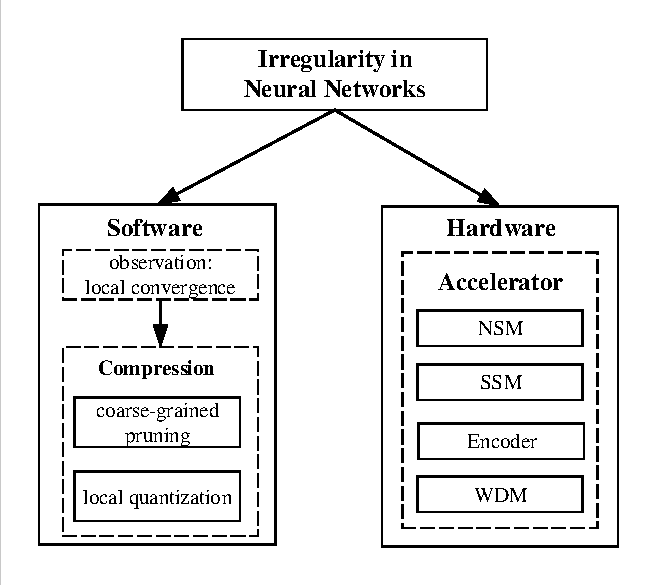
\includegraphics[width=0.8\columnwidth]{idea.pdf}
\caption{本文主要研究内容和创新点}
\label{fig:idea}
\end{figure}


最近的研究~\cite{han2015learning,han2015deep,wang2016cnnpack,zhou2017incremental}表明,神经网络可以在保持精度的前提下,通过稀疏,量化,低精度等方式进行深度压缩,从而减少参数存储量,计算量和访存量。然而,稀疏技术会使得原本规则的神经网络计算变得不规则,因此CPU,GPU以及一些不支持稀疏的加速器并不能从中受益。尽管,最近出现了一些能够支持稀疏的神经网络加速器~\cite{chen2017eyeriss,zhang2016cambricon,albericio2016cnvlutin,han2016eie,han2017ese,angshuman2017scnn},但是挖掘稀疏的效果并不理想。


本来提出了一种软硬件结合方法(software/hardware cooprative approach)来处理稀疏神经网络的不规则性。我们首先提出了粗粒度剪枝算法,从而减少稀疏神经网络的不规则性,同时对神经网络进行深度压缩。然后我们设计了粗粒度稀疏神经网络加速器来处理经过粗细度稀疏的神经网络,新型加速器有高性能和和低能耗的特点。本文的主要贡献如图~\ref{fig:idea}所示,可以归纳如下:

1.本文首次提出采用软硬件结合的方法处理稀疏神经网络不规则性。在软件方面我们提出了一种新的压缩算法对神经网络进行深度压缩,压缩算法中包含的粗粒度稀疏算法能够减少稀疏神经网络的不规则形;在硬件方面,我们提出了粗粒度稀疏神经网络加速器来高效处理粗粒度稀疏,从而获得高性能。

2. 本文观察到了局部收敛(local convergence)的现象,即神经网络的权值不是一种随机分布的情况,而是在训练过程中大的权值会聚集成簇,我们通过大量实验证明局部收敛的现象出现在许多的神经网络中。本文根据观察到的局部收敛现象,提出了一种新的神经网络压缩算法。压缩算法包括三个步骤,分别是粗粒度剪枝(coarse-grained pruning),局部量化(local quantization)和熵编码(entropy coding)。粗粒度剪枝将神经网络的权值分为多个权值块,当一个权值块符合某个条件时将从网络拓扑中被完全剪除,粗粒度稀疏的神经网络对比与细粒度稀疏的神经网络拥有更低的不规则度。局部量化将权值分为多个子区域,然后在每一个子区域内分别进行量化,进一步压缩神经网络。之后,我们采用熵编码对神经网络进行无损压缩。新的神经网络算法不仅能够降低稀疏神经网络的稀疏度,还最终获得非常理想的压缩比。

3. 本文设计并提出了首个能够支持粗粒度稀疏神经网络的加速器微结构。该微结构不仅能够处理普通的稠密神经网络,还能够通过打开/关闭稀疏处理模块支持多种稀疏/量化情况,包括神经元稀疏,粗粒度权值稀疏,神经元/权值同时稀疏情况,局部量化等。新型加速器能够非常高效的利用稀疏和量化,获得非常理想的性能和能耗。

\section{论文的组织结构}
本文第一章介绍了本文的工作背景。我们主要从神经网络算法的发展历史和神经网络加速器的发展历史两方面进行分析。

本文第二章介绍了神经网络相关的背景知识。首先我们介绍了神经网络算法,对神经网络的多种不同类型的层计算进行详细分析。然后我们介绍了神经网络的低能耗技术,包括低精度计算技术和深度压缩技术。最后我们介绍最新神经网络加速器的相关工作,其中我们重点介绍了稀疏神经网络加速器。

本文第三章提出了一种新的神经网络压缩方法。首先我们观察到神经网络的权值在训练过程中有局部收敛的现象,即大的权值容易聚集成簇。基于局部收敛,我们提出了粗粒度剪枝的策略,将多个权值同时进行剪枝剪枝操作;然后我们提出局部量化的方案进一步利用局部收敛,减少表示权值的比特数,进一步对神经网络进行压缩;最后我们利用熵编码对神经网络进行无损压缩。最后通过大量实验证明,新的压缩方法能够对神经网络进行深度压缩,同时减少稀疏神经网络的不规则性。

本文第四章提出了一个新的粗粒度稀疏神经网络加速器,能够快速处理经过深度压缩的神经网络。首先,我们观察粗粒度稀疏神经网络的特点,提出了设计加速器的三个原则。然后我们根据这三个设计原则,提出了新型加速器的架构,新的加速器能够充分利用神经元稀疏,粗粒度权值稀疏和局部量化,从而提高性能,降低功耗。最后我们为新型加速器设计了专用的编程框架,减轻用户的编程负担。

本文第五章提出了一个新型加速器专用的性能模拟器,同时完成加速器相关的性能和功耗的相关实验。首先,我们根据新型加速器的特性,设计了一个性能模拟器代替周期精确模拟器,从而在误差允许的范围内,快速完成对加速器的性能评估。然后我们对加速器进行详细的性能和能耗评估,在七个benchmark上,我们分别将新型加速器与CPU,GPU,DianNao和Cambricon-X进行比较。最后我们根据实验结果详细分析了新型加速器能够获得高性能和低能耗的原因。

最后一章我们对本文进行总结,并展望了未来的研究工作。
